\subsection{Conditional response gradients with actual fixed-Qwen researchers}
\label{sec:native-qwen-response-v9}

The scripted check above asks whether the response-boundary machinery can
represent a known adapter.  The v9 pilot instead asks a narrower empirical
question: along one observed original-native history, can a local numeric
operator fitted to actual fixed-Qwen review replies produce an auditable
institution-coordinate gradient and a precommitted native reevaluation?  The
researcher model weights remain fixed, but its replies are not frozen.  Every
endpoint executes the original two-year, five-author, seed-42 world, including
research, submission, review, publication and funding.  Thus the fitted object
is a conditional response map inside the native forward process, not a new
numeric replacement world and not a derivative of Qwen's weights or tokens.

The fixed development loss is the existing reviewed-utility proxy
\begin{equation}
  L(\theta)=3.25A(\theta)-Q(\theta)+0.05R(\theta),
  \label{eq:native-qwen-v9-loss}
\end{equation}
where $A$ is the number of accepted native decisions, $Q$ sums the arithmetic
mean of native integer-parsed reviewer scores for accepted decisions, and $R$ counts all native
review records.  No quality, fairness or participation veto is added; reject-all
remains legal.  The sole optimized institution coordinate $\theta\in[0,1]$ is
the evidence weight in a public review charter, paired with originality weight
$1-\theta$.  The charter is delivered only after year-2 research, submissions
and costs, immediately before the original review phase.  It changes actual
reviewer input text but not model weights, target scores, the original integer
parser, or the fixed addressed-selection thresholds.  A second tensor
mechanism independently accounts for the same hard native loss in
Eq.~\eqref{eq:native-qwen-v9-loss}; hard replay mismatch is an error rather than
a fit target.

\paragraph{One coupled history, then fresh affected replies.}
Independent actual-Qwen reset worlds already differed before the intervention,
so the preserved a1/a2 attempts cannot identify a controlled response effect.
They contain two complete and two partial worlds with 228 physical replies;
partial losses remain null.  The prospective a3 protocol instead seals the
complete $\theta=.2$ world as an actual-history anchor.  Each of six new native
executions replays an anchor reply only when the next original request payload,
year and seed match exactly.  For year-1 reviews, the normal review insertion
runs first, every non-clock field is checked against the anchor, and only the
operational \code{review\_time} is restored.  The first non-replayed request
must be a year-2 review; that reply and every later reply are fresh Qwen calls.
This shares one observed pre-intervention society rather than fabricating six
independent histories.  Logical replay rows retain their original request,
cache and raw-response hashes, while fresh physical calls are counted
separately.

\paragraph{Calibration-only backward and frozen proposal.}
Three declared controls $\theta\in\{.2,.5,.8\}$ fit a local raw-score response
operator.  Each review is projected separately through the original task and
record identities before paper-level averaging; missing or changed identities
are unsupported rather than padded.  Temperature is chosen from
$\{1,.2,.05,.01\}$ using calibration-loss RMSE only.  At the center, autograd
through the fitted response operator, tensor selector and native loss accounting
produces the represented gradient $\widehat g=\partial\widehat L/\partial\theta$.
The only allowed proposal is
\begin{equation}
 \theta'=\operatorname{clip}_{[.2,.8]}
 \left(.5+\operatorname{clip}_{[-.10,.10]}(-.02\widehat g)\right).
 \label{eq:native-qwen-v9-step}
\end{equation}
The operator and proposal are content-bound before the unused controls .35 and
.65 are read.  A numerically unchanged step is reported as a no-op, not rerolled
or converted into a favorable gradient.  The two unused coordinates and the
candidate then receive complete native executions under the same coupled-history
contract.

This design diagnoses raw response fit, frozen-response versus response-aware
prediction, unused-coordinate errors, finite-path agreement, hard/soft gap and
the candidate's observed native loss.  The unused coordinates are development
checks, not held-out seeds.  With one coupled history and one affected response
per task, even successful numerical agreement would not establish an exact
LLM/native Jacobian, a population expectation, uncertainty calibration,
scientific quality, causal institutional benefit or optimizer superiority.

\paragraph{Audited actual result: the loop closes, but fidelity and update fail.}
All six a3 worlds complete without technical failure (Table~\ref{tab:native-qwen-v9}).
Each executes 84 logical replies: the same 53-reply anchor prefix and 31 fresh
physical Qwen replies.  The totals are therefore 504 logical rows, 318 logical
replays and 186 new physical calls; 239 unique actual calls support a3 when the
anchor is counted once.  Including the preserved a1/a2 attempts, v9 consumed
414 physical replies.  Independent audit remeasures every checkpoint and keeps
all 101 a3 raw files unchanged.

\begin{table}[t]
\caption{Common-prefix-coupled a3 development worlds.  The predicted loss is
from the calibration-fitted response operator; lower native loss is better.
C, U and G denote calibration, unused and frozen-gradient-candidate worlds.}
\label{tab:native-qwen-v9}
\centering
\scriptsize
\begin{tabular}{lrrrrrr}
\toprule
World & $\theta$ & $A$ & $Q$ & $R$ & Native $L$ & Predicted $L$ \\
\midrule
C0 & .20 & 0 & 0     & 18 & .9000 & .9000 \\
C1 & .50 & 0 & 0     & 18 & .9000 & .9000 \\
C2 & .80 & 1 & 3.333 & 18 & .8167 & .8167 \\
U0 & .35 & 0 & 0     & 18 & .9000 & .9000 \\
U1 & .65 & 0 & 0     & 18 & .9000 & .8168 \\
G  & .50 & 0 & 0     & 18 & .9000 & .9000 \\
\bottomrule
\end{tabular}
\end{table}

Temperature .01 has calibration-loss RMSE $1.16\times10^{-5}$ and the raw
response fit has RMSE .0402.  Despite that close calibration fit, the frozen
landscape is nearly flat at the center: the represented gradient is
$1.15\times10^{-15}$.  The raw response Jacobian is learned rather than
zero-imputed; the near-zero value is the local derivative of the composed
frozen representation.  Equation~\eqref{eq:native-qwen-v9-step} therefore rounds
to the exact no-op $\theta'=.5$.  Its fresh native reevaluation has loss .9,
tying the center.  The better observed calibration endpoint, $\theta=.8$ with
loss .8167, is not retrospectively substituted for the pre-frozen gradient
proposal.  Thus the executed candidate changes no institution, and its tied
outcome cannot be attributed to an institutional update.

The unused diagnostics are a stronger negative result.  At .35, prediction
error is $2.08\times10^{-11}$; at .65 it is .08323 and fails the declared
endpoint tolerance.  Across $.35\rightarrow.65$, the native loss change is
zero.  The response-aware path predicts $-.08395$ (absolute error .08395),
whereas the frozen-response baseline predicts zero with zero error.  Hence the
response-aware representation does not improve finite-path prediction here.
The fitted model captures the lower calibration loss at .8, but its sharp
transition yields a local plateau at .5 and does not generalize to the unused
.65 endpoint (Figures~\ref{fig:native-qwen-v9-landscape} and
\ref{fig:native-qwen-v9-result}).  This is an informative implementation result:
actual response ingress, identity joins, native accounting, autograd and
reevaluation all execute, yet neither conditional fidelity nor a useful
gradient update is established.

\begin{figure}[t]
 \centering
 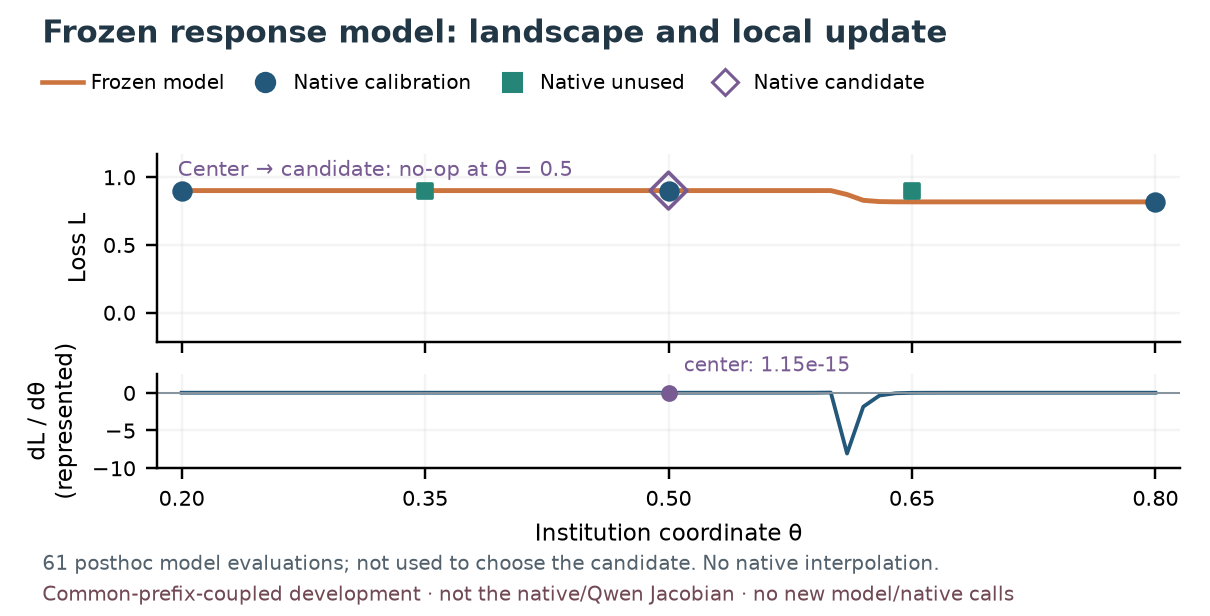
\includegraphics[width=\textwidth]{figures/native-qwen-response-v9-a3-landscape.png}
 \caption{The frozen, posthoc represented landscape and its local center
 derivative.  Native points are not interpolated, and the 61 plotted model
 evaluations start no Qwen or native calls.  Calibration point .8 is lower,
 but the precommitted center update is an exact no-op.}
 \label{fig:native-qwen-v9-landscape}
\end{figure}

\begin{figure}[p]
 \centering
 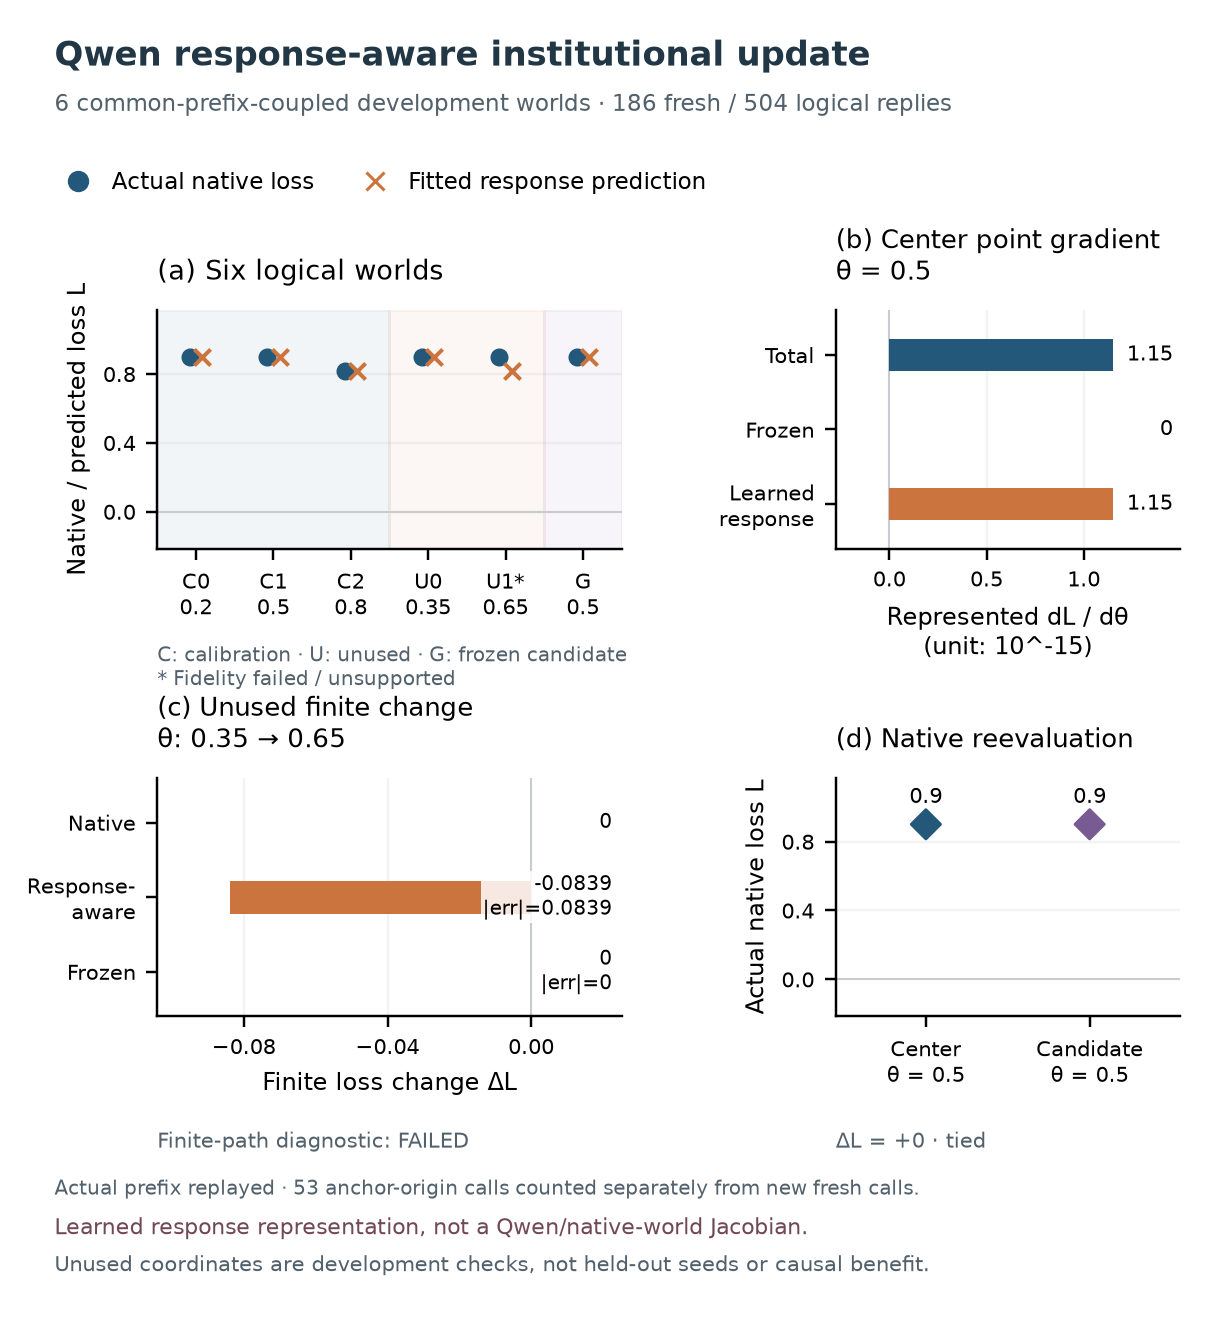
\includegraphics[width=\textwidth,height=.84\textheight,keepaspectratio]{figures/native-qwen-response-v9-a3.png}
 \caption{Actual fixed-Qwen conditional-response pilot.  The six native
 endpoints share one verified historical prefix, not six independent samples.
 The fitted operator misses the unused finite loss change and performs worse
 than the frozen-response baseline; the gradient candidate is the unchanged
 center and ties on reevaluation.  This is development evidence, not an exact
 Qwen/native Jacobian, held-out generalization or causal institutional benefit.}
 \label{fig:native-qwen-v9-result}
\end{figure}
